\SourcePage{287}{290}
\section{Permutation symmetry}

For a system consisting of only two particles, we could assert that the coordinate wave functions of stationary states, $\varphi(\mathbf r_1,\mathbf r_2)$, must be either symmetric or antisymmetric. In the general case of a system containing an arbitrary number of particles, however, the solutions of the Schrödinger equation (the coordinate wave functions) need by no means be symmetric or antisymmetric under interchange of every pair of particles, as the complete wave functions (including the spin factor) are. The reason is that interchanging only the coordinates of two particles does not yet constitute their physical interchange. The physical identity of the particles implies here only that the Hamiltonian of the system is invariant under particle interchanges; hence, if a certain function is a solution of the Schrödinger equation, then the functions obtained from it by various permutations of the variables are solutions as well.

We first make a few remarks about permutations in general. For a system of $N$ particles there are $N!$ different permutations in all. If all the particles are imagined to be numbered, each permutation can be represented by a definite sequence of the numbers $1,2,3,\ldots$ Every such sequence can be obtained from the natural sequence $1,2,3,\ldots$ by successive interchanges of pairs of particles. A permutation is called \emph{even} or \emph{odd} according as it is effected by an even or an odd number of pair interchanges. Let $\widehat P$ denote the permutation operators for $N$ particles, and introduce a quantity $\delta_P$ equal to $+1$ when $\widehat P$ is an even permutation and to $-1$ when it is odd. If $\varphi$ is symmetric in all the particles, then
\[
 \widehat P\varphi=\varphi,
\]

\SourcePage{288}{291}
whereas if the function is antisymmetric in all the particles, then
\[
 \widehat P\varphi=\delta_P\varphi.
\]

From an arbitrary function $\varphi(\mathbf r_1,\mathbf r_2,\ldots,\mathbf r_N)$ a symmetric function can be formed by the operation of \emph{symmetrization}, which may be written
\begin{equation}
 \varphi_{\text{sym}}=\operatorname{const}\cdot\sum_P\widehat P\varphi,
 \tag{63.1}
\end{equation}
where the summation extends over all possible permutations. The formation of an antisymmetric function (an operation sometimes called \emph{alternation}) can be written
\begin{equation}
 \varphi_{\text{antisym}}=\operatorname{const}\cdot\sum_P\delta_P\widehat P\varphi.
 \tag{63.2}
\end{equation}

Let us return to the behavior of the wave functions $\varphi$ of a system of identical particles under permutations\footnote{Mathematically, the problem is that of finding the irreducible representations of the permutation group. For detailed accounts of the mathematical theory of permutation groups, see: H.~Weyl, \emph{The Theory of Groups and Quantum Mechanics}; M.~Hamermesh, \emph{Group Theory and Its Application to Physical Problems}; I.~G.~Kaplan, \emph{Symmetry of Many-Electron Systems}.}. The symmetry of the system Hamiltonian $\widehat H$ in all the particles means mathematically that it commutes with every permutation operator $\widehat P$. These operators, however, do not commute with one another and therefore cannot be reduced simultaneously to diagonal form. Thus the wave functions $\varphi$ cannot be chosen so that every one of them is symmetric or antisymmetric under all the separate pair interchanges\footnote{Only for a system of two particles is there just one interchange operator, which can be reduced to diagonal form simultaneously with the Hamiltonian.}.

We shall pose the problem of determining the possible symmetry types, under permutations of the variables, of functions $\varphi(\mathbf r_1,\mathbf r_2,\ldots,\mathbf r_N)$ of $N$ variables (or of sets of several such functions).

The symmetry must be incapable of further increase: every additional operation of symmetrization or alternation applied to these functions must turn them either into linear combinations of the same functions or identically into zero.

\SourcePage{289}{292}
We already know two operations that produce functions of maximal symmetry: symmetrization in all the variables and alternation in all the variables. These operations may be generalized as follows.

Divide the set of all $N$ variables $\mathbf r_1,\mathbf r_2,\ldots,\mathbf r_N$ (or, equivalently, the indices $1,2,3,\ldots,N$) into several rows containing $N_1,N_2,\ldots$ elements (variables), where $N_1+N_2+\ldots=N$. Such a partition can be represented pictorially by a diagram (the so-called \emph{Young diagram}) in which each of the numbers $N_1,N_2,\ldots$ is represented by a row of cells (thus Fig.~21 shows the diagrams for the partitions $6+4+4+3+3+1+1$ and $7+5+5+3+1+1$ when $N=22$); one of the numbers $1,2,3,\ldots$ is to be placed in every cell. If the rows are arranged in order of decreasing length (as in Fig.~21), the diagram contains not only successive horizontal rows but also vertical columns.

\begin{figure}[ht]
\centering
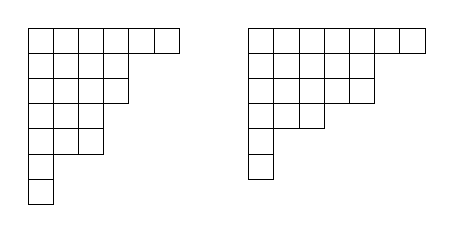
\begin{tikzpicture}[x=3.2mm,y=3.2mm,line width=.35pt]
 \foreach \r/\n in {0/6,1/4,2/4,3/3,4/3,5/1,6/1}{\foreach \c in {0,...,\numexpr\n-1\relax}{\draw (\c,-\r) rectangle ++(1,-1);}}
 \begin{scope}[xshift=28mm]
 \foreach \r/\n in {0/7,1/5,2/5,3/3,4/1,5/1}{\foreach \c in {0,...,\numexpr\n-1\relax}{\draw (\c,-\r) rectangle ++(1,-1);}}
 \end{scope}
\end{tikzpicture}
\par\smallskip {\small Fig. 21}
\end{figure}

Symmetrize an arbitrary function $\varphi(\mathbf r_1,\mathbf r_2,\ldots,\mathbf r_N)$ in the variables belonging to each row. After this, alternation can be carried out only with respect to variables belonging to different rows; alternation in a pair of variables lying in the same row would plainly give zero identically.

Select one variable from each row; without loss of generality, these may be regarded as occupying the first cells of the rows (after symmetrization, the order of the variables among the cells of each row is immaterial), and perform alternation in these variables. Next remove the first column and perform alternation in the variables selected one from each row of the diagram thus shortened; these variables may again be regarded as occupying the first cells of the shortened rows. Continuing this procedure, we obtain a function first symmetrized in the variables of each row and then alternated in the variables of each column (after alternation the function, of course, is in general no longer symmetric in the variables of each row; symmetry is retained only with respect to the variables in the cells of the first row that project beyond the other rows).

By distributing the $N$ variables among the rows of a Young diagram in different ways (their distribution among the cells of each row

\SourcePage{290}{293}
being immaterial), we obtain in this way a set of functions that transform into one another under arbitrary permutations of the variables\footnote{Symmetrization and alternation could instead be performed in the reverse order---first alternating in the variables of each column and then symmetrizing in those of the rows. This would yield nothing new, however, since the functions obtained by the two procedures are linear combinations of one another.}. It must be stressed, however, that not all these functions are linearly independent; in general the number of independent functions is smaller than the number of possible distributions of the variables among the rows of the diagram. We shall not discuss this point further here\footnote{The independent functions that transform into one another form a basis of an irreducible representation of the permutation group. Their number is the dimension of the representation. For particles of spin $1/2$, it is found in Problem 1 of this section.}.

Thus every Young diagram determines a certain symmetry type of functions under permutations. By constructing all the Young diagrams possible for a given $N$, we find all possible symmetry types. This amounts to partitioning the number $N$ in every possible way into a sum of smaller terms, with $N$ itself also counted among the possible partitions (for $N=4$, for example, the partitions are $4$, $3+1$, $2+2$, $2+1+1$, and $1+1+1+1$).

To each energy level of the system there can be assigned a Young diagram determining the permutation symmetry of the corresponding solutions of the Schrödinger equation; in general, several different functions correspond to each energy value and transform into one another under permutations. This ``permutation degeneracy'' is associated with the noncommutativity, already mentioned, of the operators $\widehat P$, each of which commutes with the Hamiltonian (cf. §~10, p.~48). It should be stressed, however, that this does not signify any additional physical degeneracy of the energy levels. All these different coordinate wave functions, multiplied by spin functions, enter into a single definite combination---the complete wave function---which satisfies, according to the spin of the particles, the condition of symmetry or antisymmetry.

Among the different symmetry types there are always two (for a given $N$) to which only one function apiece corresponds. One is represented by a function symmetric in all the variables, and the other by an antisymmetric function (in the former case

\SourcePage{291}{294}
the Young diagram consists of a single row of $N$ cells, and in the latter of a single column).

We turn now to the spin wave functions $\chi(\sigma_1,\sigma_2,\ldots,\sigma_N)$. Their symmetry types under particle permutations are determined by the same Young diagrams, with the particle spin projections playing the role of the variables. The question arises which diagram should correspond to the spin function for a specified diagram of the coordinate function. Suppose first that the particles have integral spin. The complete wave function $\psi$ must then be symmetric in all particles. For this to hold, the symmetries of the spin and coordinate functions must be described by the same Young diagram, and the complete wave function $\psi$ is expressed as certain bilinear combinations of the two; we shall not consider here how this combination is constructed.

Suppose next that the particles have half-integral spin. The complete wave function must then be antisymmetric in all the particles. It can be shown that the Young diagrams of the coordinate and spin functions must consequently be dual: one is obtained from the other by interchanging rows and columns (the two diagrams shown in Fig.~21 are an example).

We examine in more detail the important case of particles of spin $1/2$ (electrons, for example). Each spin variable $\sigma_1,\sigma_2,\ldots$ then takes only the two values $\pm1/2$. Since a function antisymmetric in any two variables vanishes when those variables have equal values, it is clear that $\chi$ can be alternated only in pairs of variables; if alternation is performed in three variables, two of them must have equal values, and the result is identically zero.

Thus, for a system of electrons, the Young diagrams of the spin functions can have columns only one or two cells long (that is, only one or two rows in all); in the Young diagrams of the coordinate functions, the same restriction applies to the row lengths. The number of possible permutation-symmetry types for a system of $N$ electrons is consequently the number of ways of partitioning $N$ into a sum of ones and twos. For even $N$ this number is $N/2+1$ (the partitions with $0,1,\ldots,N/2$ twos), and for odd $N$ it is $(N+1)/2$ (the partitions with $0,1,\ldots,(N-1)/2$ twos). Figure~22 shows, for example, the possible Young diagrams (coordinate and spin) for $N=4$.

It is readily seen that each of these symmetry types (that is, each Young diagram) corresponds to a definite total spin $S$ of the electron system. We shall write

\SourcePage{292}{295}
the spin functions in spinor form, namely as a spinor $\chi^{\lambda\mu\ldots}$ of rank $N$, whose indices (each corresponding to the spin of a separate particle) are the variables placed in the cells of the Young diagrams.

\begin{figure}[ht]
\centering
\begin{tikzpicture}[x=5mm,y=5mm,line width=.35pt]
 \node[anchor=east] at (-0.5,-0.5) {$\varphi$};
 \node[anchor=east] at (-0.5,-2.5) {$\chi$};
 %% phi diagrams: 1-column, 2+1, 2+2
 \foreach \r in {0}{\draw (0,-\r) rectangle ++(1,-1);}
 \foreach \r/\n in {0/1,1/1}{\foreach \c in {0,...,\numexpr\n-1\relax}{\draw (3+\c,-\r) rectangle ++(1,-1);}}
 \foreach \r/\n in {0/2}{\foreach \c in {0,...,\numexpr\n-1\relax}{\draw (6+\c,-\r) rectangle ++(1,-1);}}
 %% chi diagrams (dual): 4-column, 3+1, 2+2
 \foreach \c in {0,...,3}{\draw (\c,-2) rectangle ++(1,-1);}
 \foreach \r/\n in {0/2,1/1,2/1}{\foreach \c in {0,...,\numexpr\n-1\relax}{\draw (3+\c,-2-\r) rectangle ++(1,-1);}}
 \foreach \r/\n in {0/2,1/2}{\foreach \c in {0,...,\numexpr\n-1\relax}{\draw (6+\c,-2-\r) rectangle ++(1,-1);}}
 %% combined S-diagrams
 \foreach \c in {0,...,3}{\draw (\c,-6) rectangle ++(1,-1);}
 \node at (2,-7.7) {$S=2$};
 \foreach \r/\n in {0/3,1/1}{\foreach \c in {0,...,\numexpr\n-1\relax}{\draw (5+\c,-6-\r) rectangle ++(1,-1);}}
 \node at (6.5,-8.8) {$S=1$};
 \foreach \r/\n in {0/2,1/2}{\foreach \c in {0,...,\numexpr\n-1\relax}{\draw (10+\c,-6-\r) rectangle ++(1,-1);}}
 \node at (11,-8.8) {$S=0$};
\end{tikzpicture}
\par\smallskip {\small Fig. 22}
\end{figure}

Consider a spin Young diagram consisting of two rows with $N_1$ and $N_2$ cells ($N_1+N_2=N$, $N_1\geq N_2$). Each of the first $N_2$ columns contains two cells, and the spinor must be antisymmetric in the corresponding pairs of indices. It must be symmetric, on the other hand, in the indices occupying the last $n=N_1-N_2$ cells of the first row. As we know, however, such a spinor of rank $N$ reduces to a symmetric spinor of rank $n$, corresponding to the total spin $S=n/2$. Returning to the Young diagrams of the coordinate functions, we can say that the diagram with $n$ rows containing one cell each corresponds to a state of total spin $S=n/2$. For even $N$ the total spin can take the integral values from 0 to $N/2$, and for odd $N$ the half-integral values from $1/2$ to $N/2$, as it should.

It should be emphasized that this one-to-one correspondence between Young diagrams and total spin occurs only for systems of particles with spin $1/2$; for a system of just two particles we already saw it in the preceding section. For a system of $N$ particles of spin $s$, the spin wave function is constructed from a product of $N$ symmetric spinors of rank $2s$, and is therefore a spinor of rank $2Ns$. If this spinor is symmetrized according to a given Young diagram of $N$ cells, its independent components can usually be combined into several sets of linear combinations, each corresponding to a different value of the total spin $S$ of the system.

Just as the Young diagram of the spin functions for particles of spin $1/2$ cannot contain columns of more than two cells, for particles of arbitrary spin $s$ the column length cannot exceed $2s+1$ cells.

If the number $N$ of particles in the system is an integral multiple of $2s+1$, the possible Young diagrams include a rectangular one in which every column contains $2s+1$ cells. This diagram corresponds to one definite value of the total spin, $S=0$. It follows that any two (spin) Young diagrams that can be fitted together to form a rectangle

\SourcePage{293}{296}
of height $2s+1$ correspond to the same values of $S$\footnote{For example, the following pairs of diagrams have this property (for $s=1$):
\begin{center}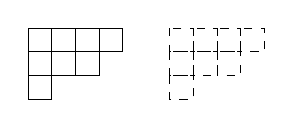
\begin{tikzpicture}[x=3mm,y=3mm,line width=.35pt]
\foreach \r/\n in {0/4,1/3,2/1}{\foreach \c in {0,...,\numexpr\n-1\relax}{\draw (\c,-\r) rectangle ++(1,-1);}}
\foreach \r/\n in {0/4,1/3,2/1}{\foreach \c in {0,...,\numexpr\n-1\relax}{\draw[dashed] (6+\c,-\r) rectangle ++(1,-1);}}
\end{tikzpicture}\end{center}
Mutually complementary diagrams are shown by solid and dashed lines.}. This conclusion is simply a consequence of the fact that the resultant of two angular momenta can be zero only when the angular momenta being added have equal magnitudes.

To conclude this section, we return to the fact noted earlier (see the note on p.~86) that, for systems of several identical particles, it cannot be asserted that the stationary-state wave function of lowest energy has no nodes. We can now make this statement more precise and explain its origin.

A wave function (here the coordinate function is meant) having no nodes must be symmetric in all the particles; if it were antisymmetric under interchange of any pair of particles 1 and 2, it would vanish when $\mathbf r_1=\mathbf r_2$. But if the system consists of three or more electrons, a completely symmetric coordinate wave function is not allowed at all (the Young diagram of the coordinate function cannot have rows of more than two cells). Thus, although the solution of the Schrödinger equation corresponding to the lowest eigenvalue has no nodes (by the theorem of the calculus of variations), this solution may be physically inadmissible. The normal state of the system then corresponds not to the lowest eigenvalue of the Schrödinger equation, and the wave function of this state will in general have nodes. More generally, for particles of half-integral spin $s$, this situation occurs in systems of more than $2s+1$ particles. For systems consisting of bosons, however, a completely symmetric coordinate wave function is always possible.
